\section{Advanced operational amplifier applications}

	\subsection{Categories of ideal operational amplifiers}
		\begin{table}[htbp]
			\centering
			\begin{tabularx}{0.9\linewidth}{lXX} \toprule
				& Voltage output & Current output \\ \midrule
					Voltage input 
				& 
					Normal Op-Amp \newline 
					$U_a = A_D U_D$ \newline 
					\begin{center}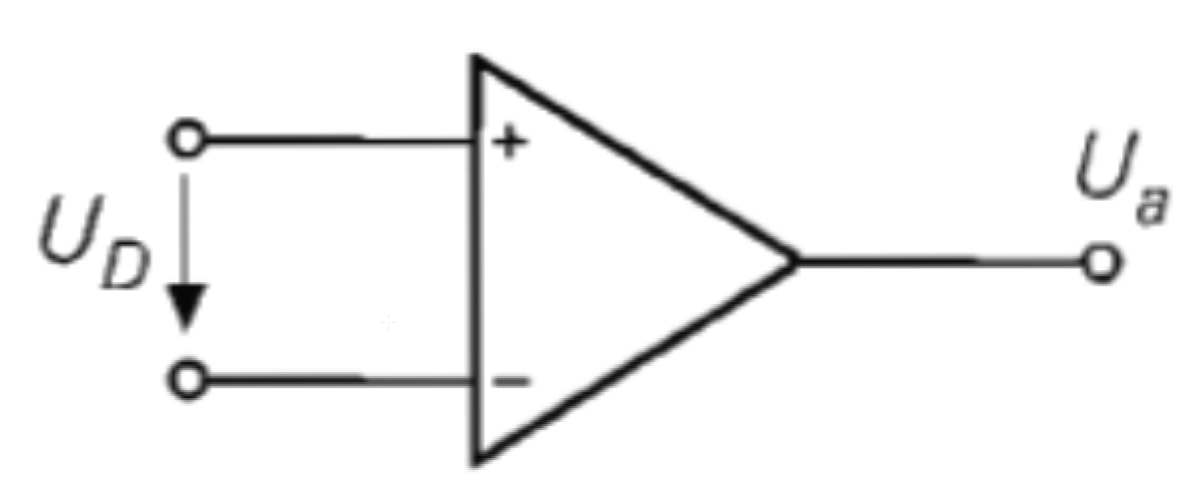
\includegraphics[width=0.25\textwidth]{images/NormalOPAMP.png}\end{center}  
				& 	Transconductance Op-Amp \newline 
					$I_a = S_D U_D$ \newline
					\begin{center}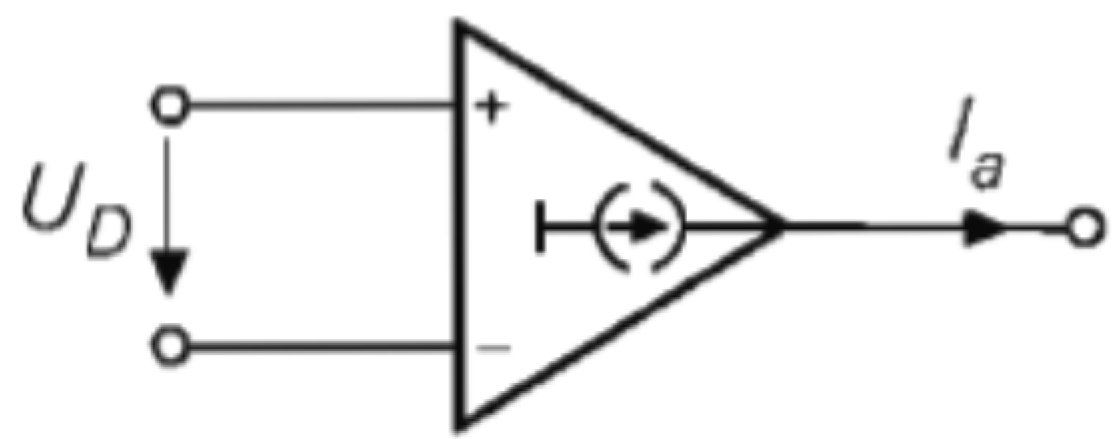
\includegraphics[width=0.25\textwidth]{images/TransconductanceOPAMP.png}\end{center}
				\\
					Current input 
				& 	Transimpedance Op-Amp \newline 
					$U_a = Z I_N$\newline
					\begin{center}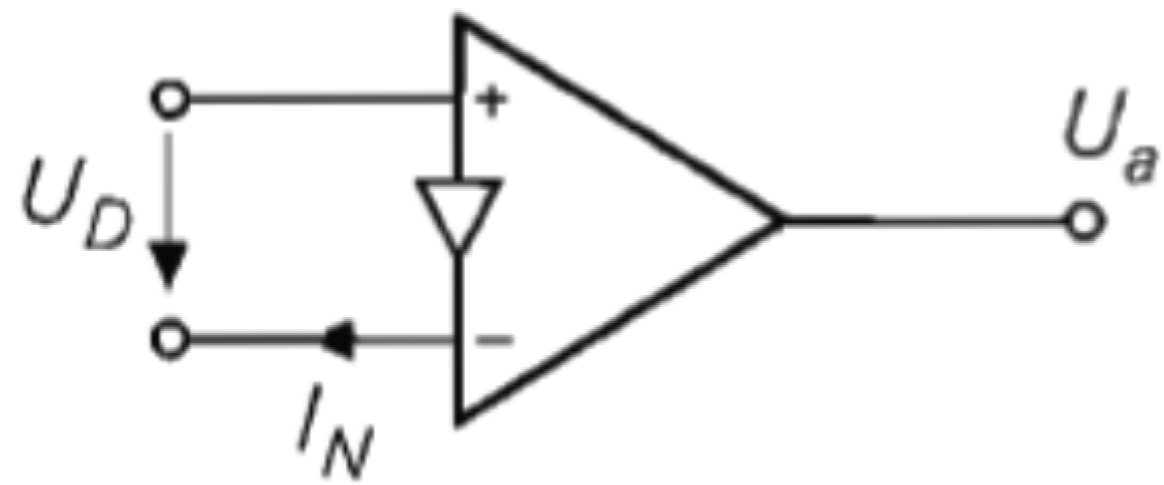
\includegraphics[width=0.25\textwidth]{images/TransimpedanceOPAMP.png}\end{center}
				 & 	Current Op-Amp \newline 
				 	$I_a = k I_N$\newline
				 	\begin{center}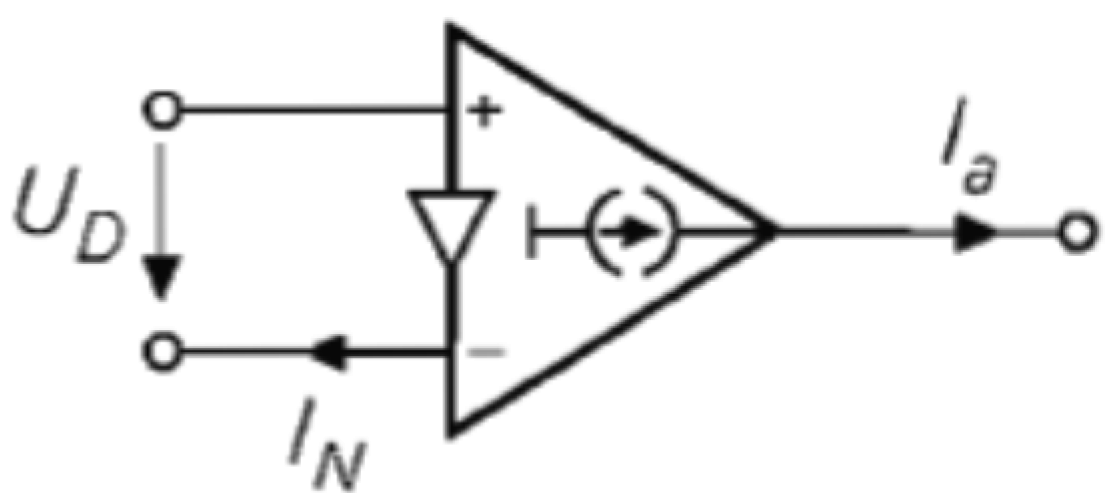
\includegraphics[width=0.25\textwidth]{images/CurrentOPAMP.png}\end{center} \\ \bottomrule
			\end{tabularx}
		\end{table}
	
	
	\subsection{Control loop block diagram}
		\begin{figure}[h]
			\centering
			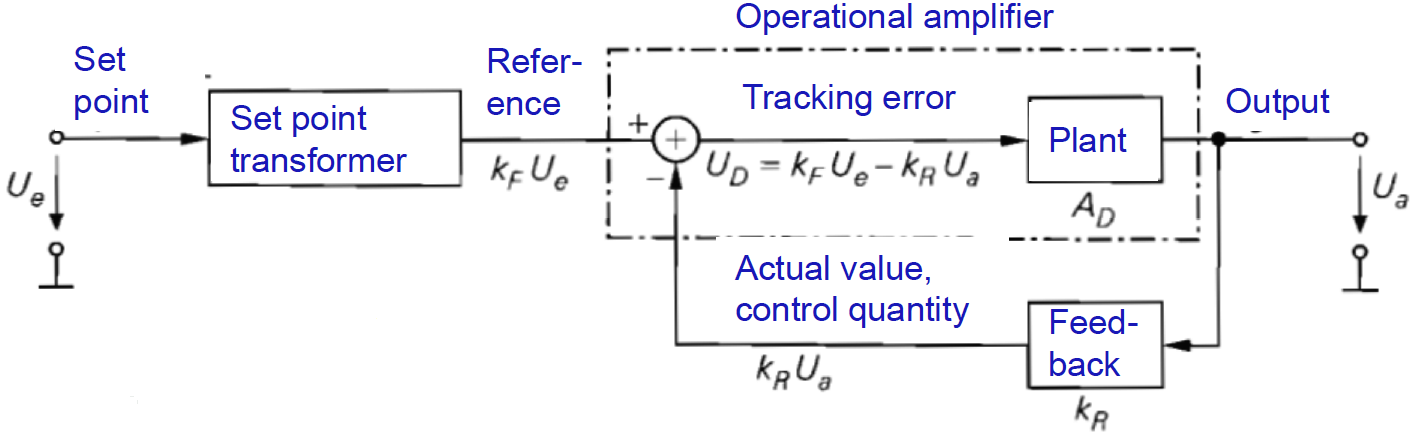
\includegraphics[width=0.75\textwidth]{images/ControlLoopDiagram.png}
			\caption{Control Loop Block Diagram}
			\label{Fig:ControlLoopDiagram}
		\end{figure}
	
		\begin{table}[htbp]
			\centering
			\begin{tabular}{llll}
				Open-loop gain & $A_D$ & Closed-loop gain & $A$\\
				Feedback loop gain & $g$ & Feedback factor & $k_R$\\
			\end{tabular}
		\end{table}
		
		\begin{align}
			U_D &= k_F U_e - k_R U_a \\
			A &= \frac{U_a}{U_e} = \frac{k_F A_D}{1 + k_R A_D} \cong \frac{k_F}{k_R}
		\end{align}
	
	\subsubsection{Non-inverting amplifier}
		\begin{figure}[h]
			\centering
			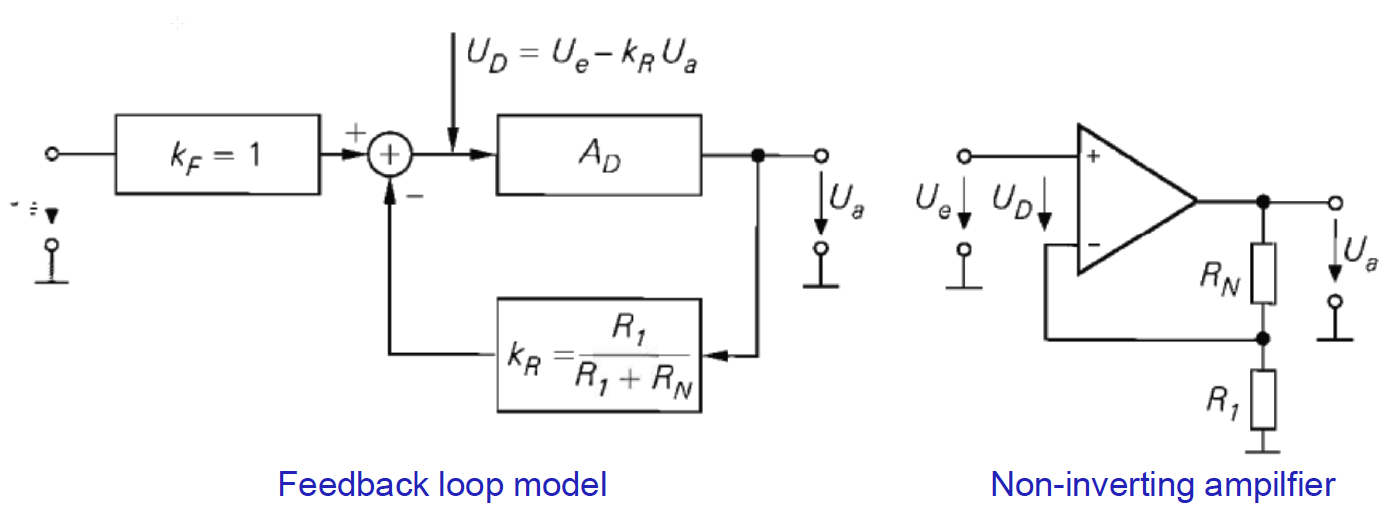
\includegraphics[width=0.75\textwidth]{images/ControlLoopNonInvertingDiagram.png}
			\caption{Control Loop Block Diagram of non-inverting amp}
			\label{Fig:ControlLoopNonInvertingDiagram}
		\end{figure}
		\begin{align}
			k_F &= 1 \\
			k_R &= \frac{R_1}{R_1 + R_N} \\
			A &= \frac{U_a}{U_e} = \frac{A_D}{1 + k_R A_D} \cong \frac{1}{k_R} = 1 + \frac{R_N}{R_1}
		\end{align}
		\begin{itemize}
			\setlength{\itemsep}{-5pt}
			\item Simpflication only valid if loop gain $g = k_R A_D$ is very high. 
			\item Distinguish between:
			\item[] Open loop gain \textbf{$A_D$}
			\item[] Closed loop gain \textbf{$A$}
			\item[] Feedback loop gain \textbf{$g$}
			\item[] Feedback factor \textbf{$k_R$ }
		\end{itemize}
	\subsubsection{Inverting amplifier}
		\begin{figure}[h]
			\centering
			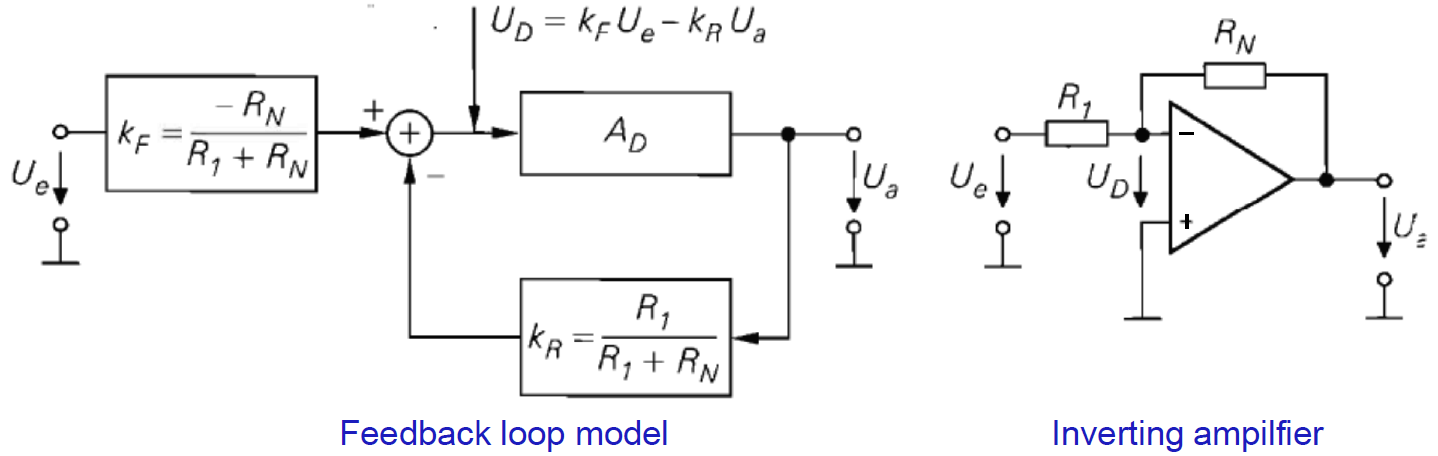
\includegraphics[width=0.75\textwidth]{images/ControlLoopInvertingDiagram.png}
			\caption{Control Loop Block Diagram of inverting amp}
			\label{Fig:ControlLoopInvertingDiagram}
		\end{figure}
		\begin{align}
			k_F &= -\frac{R_N}{R_1 + R_N} \\
			k_R &= \frac{R_1}{R_1 + R_N} \\
			A &= \frac{U_a}{U_e} \cong -\frac{R_N}{R_1}
		\end{align}
	
	\newpage
	\subsubsection{Differential amplifier}
			\begin{figure}[h]
				\centering
				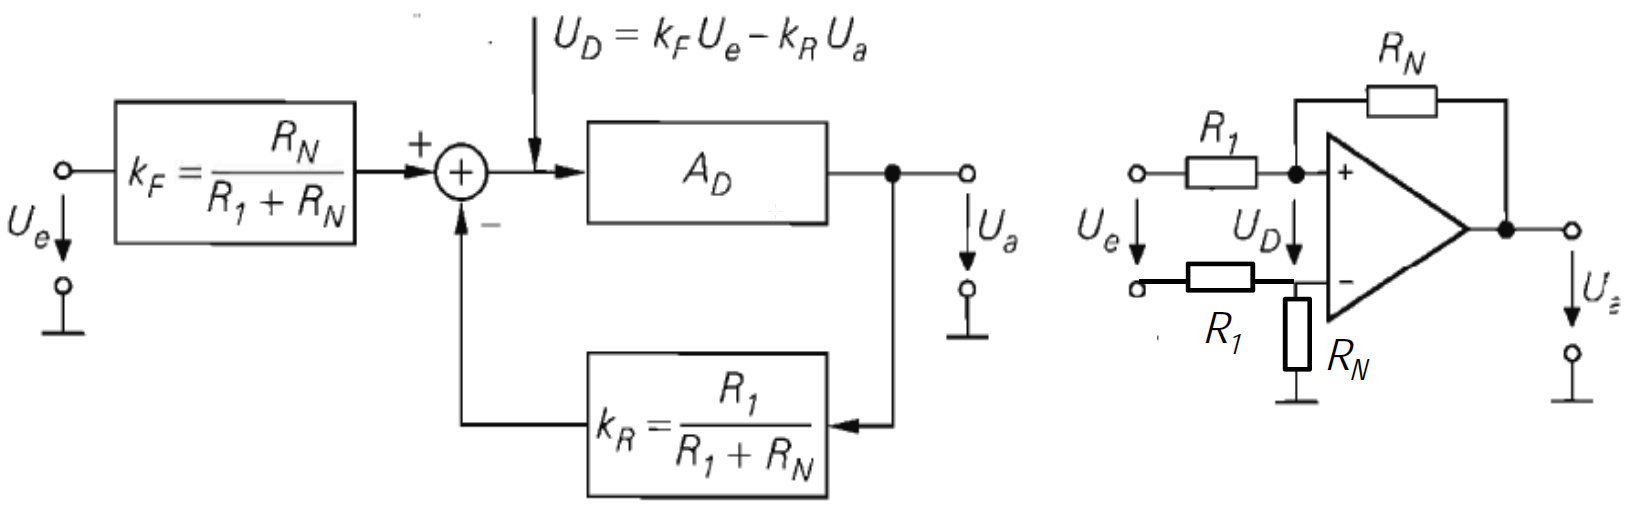
\includegraphics[width=0.75\textwidth]{images/ControlLoopDiffDiagram.png}
				\caption{Control Loop Block Diagram of differential amp}
				\label{Fig:ControlLoopDiffDiagram}
			\end{figure}
		    \begin{align}
		    	k_F &= ...\\
		    	k_R &= \\
		    	A &=  \\
		    	U_a &= \frac{R_N}{R_1}\left(U_{e+}-U_{e-}\right)
		    \end{align}
	
	\subsection{Op-Amp building blocks}
		\subsubsection{Differential pair}
			Large signal analysis: \\
			\begin{table}[h!]
				\centering
				\begin{tabular}{m{0.45\textwidth} m{0.35\textwidth} }
					
					\begin{center}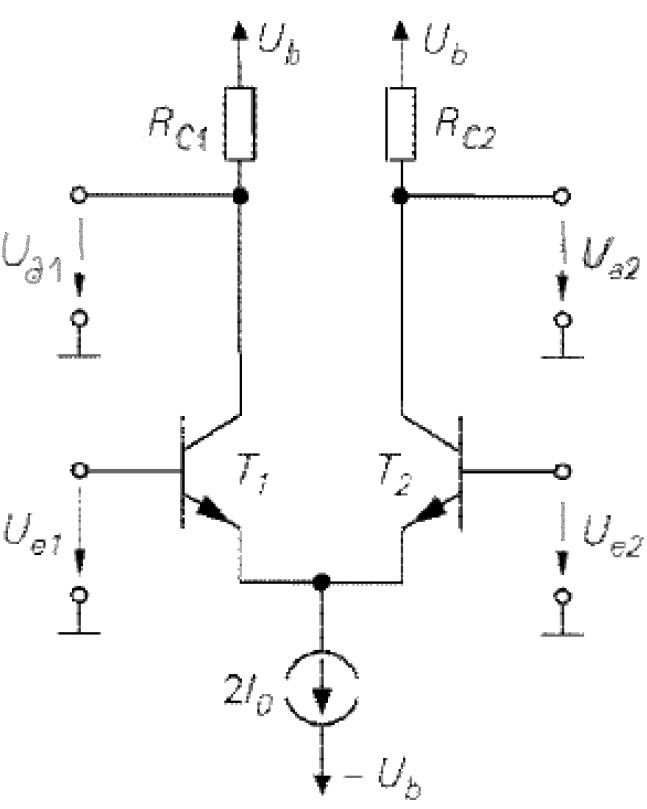
\includegraphics[width=0.25\textwidth]{images/Differenzverstaerker.png}\end{center} 
				&
							
					$I_{C1} = I_0 + \Delta I = I_0 \left( 1 + \tanh\frac{U_D}{2 U_T} \right)$\newline
					$I_{C2} = I_0 - \Delta I = I_0 \left( 1 - \tanh\frac{U_D}{2 U_T} \right)$

				\\
			
				\end{tabular}
			\end{table}			
		
		
			Small signal analysis, for $R_E >> r_S$ : \\
			\begin{table}[h!]
				\centering
				\begin{tabular}{m{0.45\textwidth} m{0.35\textwidth} }
					
					\begin{center}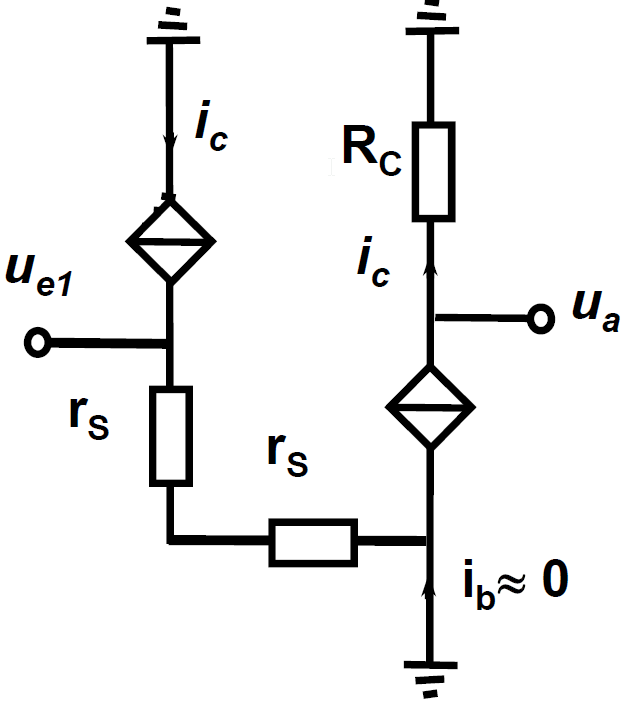
\includegraphics[width=0.25\textwidth]{images/Differenzverstaerker2.png}\end{center} 
				&
							
					$\frac{u_a}{u_{e1}} = \frac{R_C}{2 r_S}$\newline
					$\frac{u_a}{u_{e2}} = -\frac{R_C}{2 r_S}$

				\\
			
				\end{tabular}
			\end{table}				

	
		\subsubsection{Current mirror}
			\begin{multicols}{2}
				\begin{center}
					\begin{circuitikz}[scale=0.8,transform shape]
	\draw 
		(0,0) node[anchor=east] {$U_b$} to[R=$R_V$] (2,0)
		(3,-1) node[npn,xscale=-1] (t1) {}
		(6,-1) node[npn] (t2) {}
		(2,0) -| (t1.C)
		(2,0) -| (t1.B)
		(t1.B) -- (t2.B)
		(7,0) -| (t2.C)
		(t1.E) to[R=$R_1$] (3,-3.5) to (3,-4) node[rground] {}
		(t2.E) to[R=$R_2$] (6,-3.5) to (6,-4) node[rground] {}
	;		
\end{circuitikz}
				\end{center}
				\vfill
				\columnbreak
				The emitter current $I_e$ of $T1$ is
				\begin{align}
					I_e = \frac{U_b - U_{BE1}}{R_V + R_1}
				\end{align}
				The output resistance is
				\begin{align}
					r_a = \left.\frac{u_a}{i_a}\right|_{i_e=0} \cong r_{CE2} \left( 1 + \frac{\beta R_2}{R_1 + R_2 + r_{BE2}} \right)
				\end{align}
			\end{multicols}
			
			The current mirror is used as current source and active load in differential pairs to replace the resistors. 
			It allows to achieve high gains at low supply voltage.
		
		\newpage
		\subsubsection{Cascode circuit}
			Current mirror with cascode circuit increases the output resistance. 
			\begin{multicols}{2}
				\begin{center}
					\begin{circuitikz}[scale=0.8,transform shape]
	\draw 
		(0,0) node[npn] (t2) {$T_2$}
		(0,-2) node[npn] (t1) {$T_1$}
		(0,3) node[anchor=south] {$U_b$} to[R=$R_C$] (t2.C) (0,1) -- (1.5,1) node[anchor=west] {$U_a$}
		(t2.E) -- (t1.C)
		(t1.E) -- (0,-3) node[rground] {}
		(-2,-2) node[anchor=east] {$U_e$} -- (t1.B)
		(-2,0) node[anchor=east] {$U_0$} -- (t2.B)
	;
\end{circuitikz}
				\end{center}
				\vfill
				\columnbreak
				$T_1$ is in common emitter, $T_2$ in common base.
				\begin{align}
					A &= \frac{u_a}{u_e} = A_E \frac{r_{e,B}}{r_{a,E} + r_{e,B}} A_B \nonumber \\
					 &= -\frac{r_{CE1}}{r_{S1}} \frac{r_{S2}}{r_{CE1}+r_{s2}} \frac{R_C}{r_{s2}} \cong - \frac{R_C}{r_{s1}}
				\end{align}
				While the gain is identical, the output resistance is higher and the emitter stage has only gain $-1$ and thus only has a Miller capacitance of
				\begin{align}
					C_e = C_M \left( 1 + |A_{E,op}| \right) \cong 2 C_M
				\end{align}
			\end{multicols}
			
			Figure below shows a comparison about the improvements obtained by using active load and cascode circuits with regard to the static gain and the bandwidth. \\
			$\rightarrow$ More gain \& more bandwidth!
			\begin{figure}[h]
				\centering
				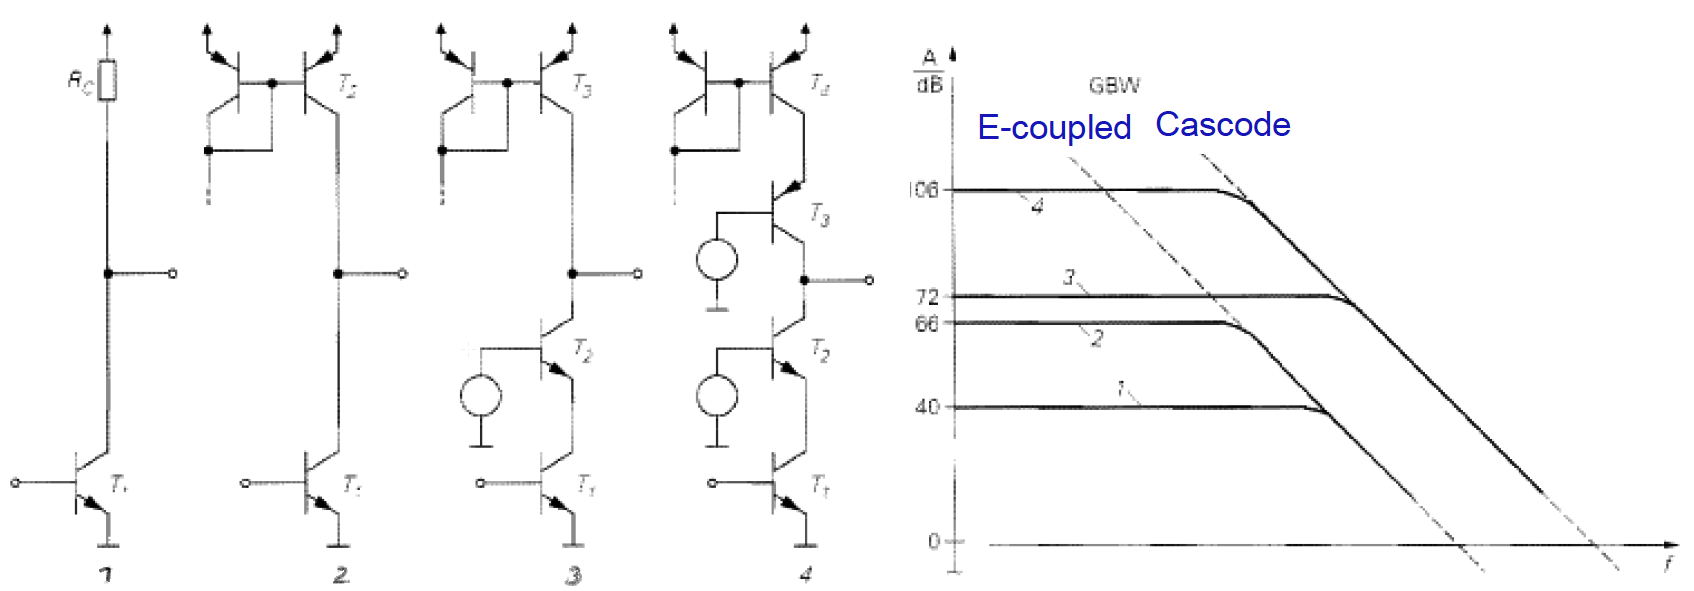
\includegraphics[width=0.75\textwidth]{images/Comparison.png}
				\caption{}
				\label{Fig:Comparison}
			\end{figure}\\
			The gain and boarder frequency (Assuming $R_B = \infty$ for border frequency: Current input) are:
			
			$A_1 = -R_C/r'_E \quad A_2 = -r_{CE}/r'_E \quad A_3 = -r_{CE}/r'_E \quad A_2 = -\beta r_{CE}/r'_E$\\
			$f_{c1} = \frac{1}{2 \pi \beta r'_E A_1 C_M} \quad f_{c1} = \frac{1}{2 \pi \beta r'_E A_2 C_M} \quad f_{c1} = \frac{1}{2 \pi \beta r'_E 2 C_M}\quad f_{c1} = \frac{1}{2 \pi \beta r'_E 2 C_M}$
			
			See also Slides 14 to 16 in OPAMP1 for further info about the cascode circuit. 

		\subsubsection{Level Shifting}
			Level shifting can be accomplished by either using Z-Diode or complementary transistors or very fancy circuit with current mirror. 
			See pages 21 to 24 in OPAMP1 for further info. 
			
		\subsubsection{Darlington Transistor}
			Advantages: \\
			Strong increase of current gain and input resistance as compared to single transistor. 
			See pages 27 in OPAMP1 for schematic. 
			
		\subsubsection{Supply Voltages}
			Rail-To-Rail OPAMP do not have a dropout voltage, meaning their signals can reach the maximum and the minimum of the supply voltage. Normal OPAMPs do have a dropout voltage. \\
			$\rightarrow$ Single Supply Amplifier LM324 see slide 31 of OPAMP1! \\
			$\rightarrow$ Single Supply CMOS AMP slide 33 of OPAMP1\\
			$\rightarrow$ Rail-To-Rail I/O OPAMP slide 35 of OPAMP1
	
	\subsection{Noise}
		Noise signals are random signals. They are aperiodic, instantaneous values which can never be predicted. The signal to noise ratio is given by
		\begin{equation}
			\frac{S}{N} = \frac{rms signal voltage}{rms noise voltage}.
		\end{equation}
		\\
		Noise can be characterized by histograms (e.g. Gauss curve) or power density spectra (e.g. uniform). In order to add independent random signals the following formula has to be used: 
		\begin{equation}
			E_{totalRMS} = \sqrt{e_{1RMS}^2 + e_{2RMS}^2 + ... + e_{nRMS}^2}
		\end{equation}
		\\
		The spectral density of noise is given in units of $\frac{V_{rms}}{\sqrt{Hz}}$ or $\frac{A_{rms}}{\sqrt{Hz}}$, whereas the power spectral density is given in $\frac{V}{Hz}$ or $\frac{A}{Hz}$ referenced to a 1 $\Omega$ resistor. \\
		\subsubsection{Corner Frequency in OPAMP noise}
			The following plot shows an example for an input noise voltage. One can see that the noise is uniform above $f_{nc}$ and 1/f below that frequency. 
			
			\begin{figure}[h]
				\centering
				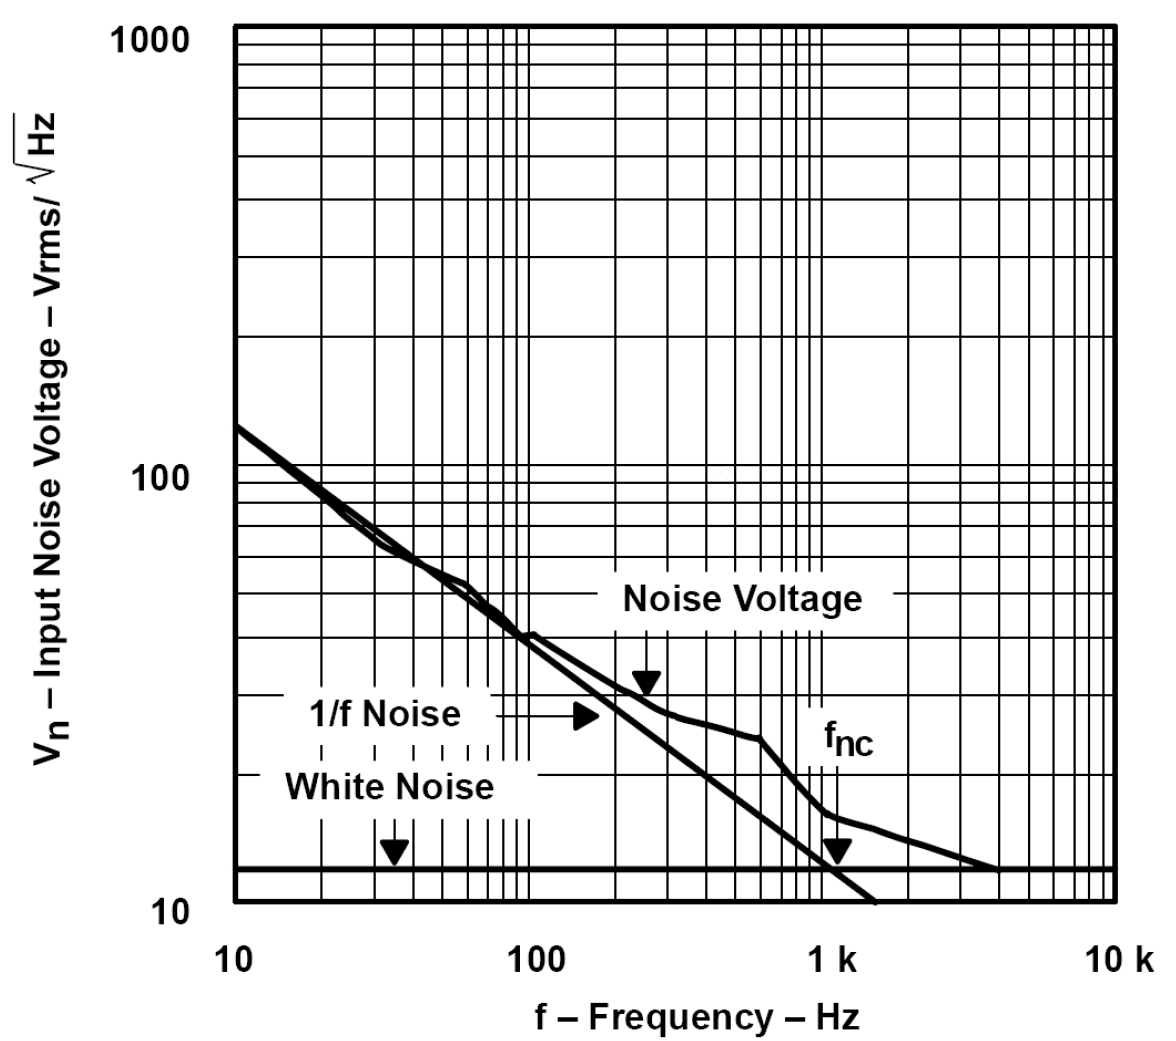
\includegraphics[width=0.45\textwidth]{images/NoiseExample.png}
				\caption{Example for input noise voltage}
				\label{Fig:NoiseExample}
			\end{figure}
			Example for computing the corner frequency $f_{nc}$:\\
			Given a noise density of 130 $\frac{nV}{\sqrt{Hz}}$ at 10 Hz and a white noise density of 12 $\frac{nV}{\sqrt{Hz}}$. \\
			On the 1/f noise power curve the product (frequency x noise power density is constant):\\
			$\left[\left(\frac{130 nV}{\sqrt{Hz}}\right)^2 - \left(\frac{12 nV}{\sqrt{Hz}}\right)^2\right]\cdot 10Hz = 167'560 nV^2$\\
			At $f_{nc}$ the noise power density is 12 $\frac{nV}{\sqrt{Hz}}$ $\rightarrow$ $\frac{167'560 nV^2}{\left(\frac{12nV}{\sqrt{Hz}}\right)^2} = 1164 Hz$
	
			Example for determining the total noise within a given bandwidth:\\
			B = $f_{min}$ to $f_{max}$\\
			Method: Noise voltage is root of noise power, therefore first integrate power and then determine the voltage. \\
			$E_n = E_{whitenoise} \cdot \sqrt{f_{nc}\cdot \ln\left(\frac{f_{max}}{f_{min}}\right) + \left(f_{max}-f_{min}\right)}$\\
		\subsubsection{Noise sources in non-inverting OPAMP}	
			An real OPAMP has - next to other errors like bias and offsets - also noise sources. The different noise sources can be added with superposition, but be aware, that the different noise contributions will be added geometrically!\\
			
			\begin{figure}[h]
				\centering
				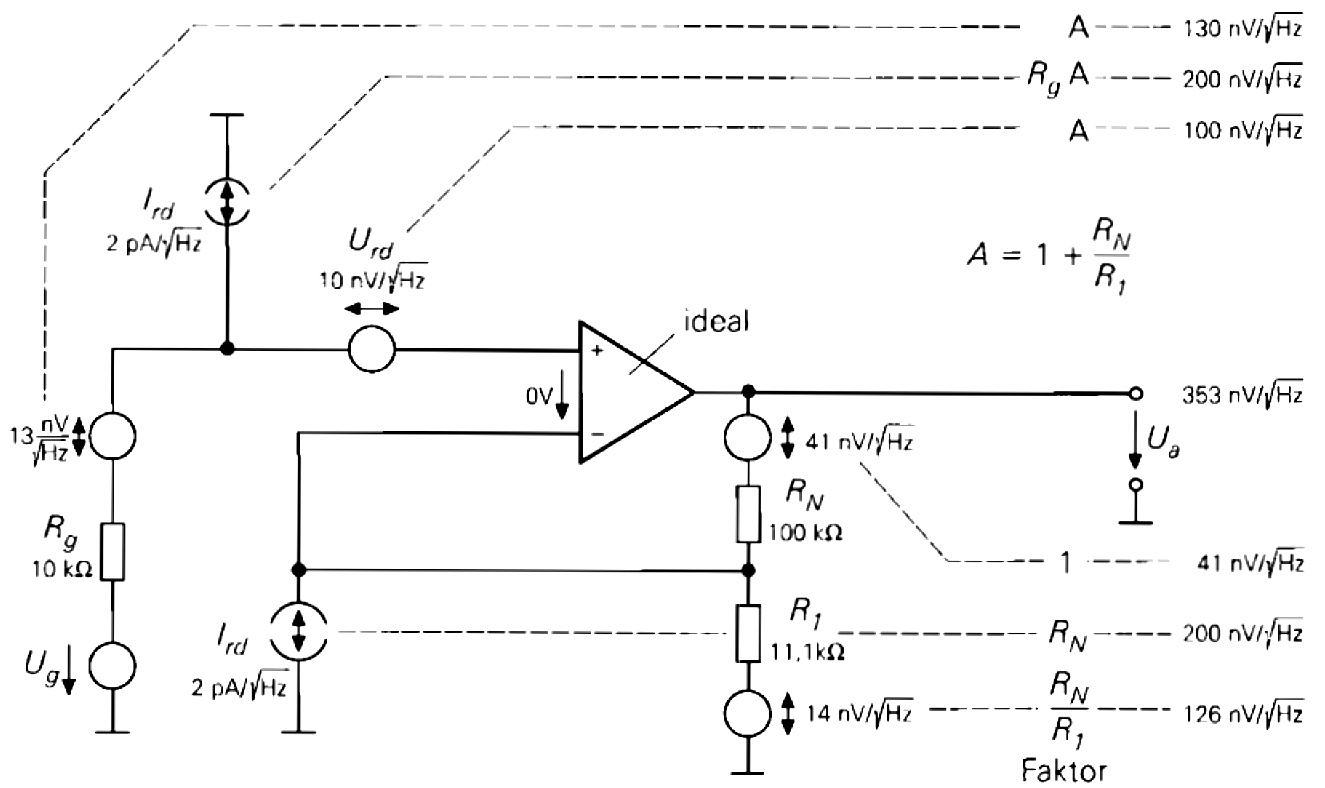
\includegraphics[width=0.65\textwidth]{images/NoiseSources.png}
				\caption{Noise sources in a non-inverting amplifier}
				\label{Fig:NoiseSources}
			\end{figure}
			The resistor noise is computed with the following formula, where $k = 1.38 \cdot 10^{-23} J/K$ is the Boltzmann constant. 
			\begin{equation}
				U_R = \sqrt{4kTR\left(f_{max}-f_{min}\right)}
			\end{equation}
		\subsubsection{Noise Voltage and Noise Number}
			The noise number is calculated by
			\begin{equation}
				F = \left(\frac{U_{outRealAMP}}{U_{outIdealAMP}}\right)^2
			\end{equation}	
			
			At low source resistance the input referred voltage noise dominate whereas at high $R_g$ the current noise dominates. 
			\begin{figure}[h]
				\centering
				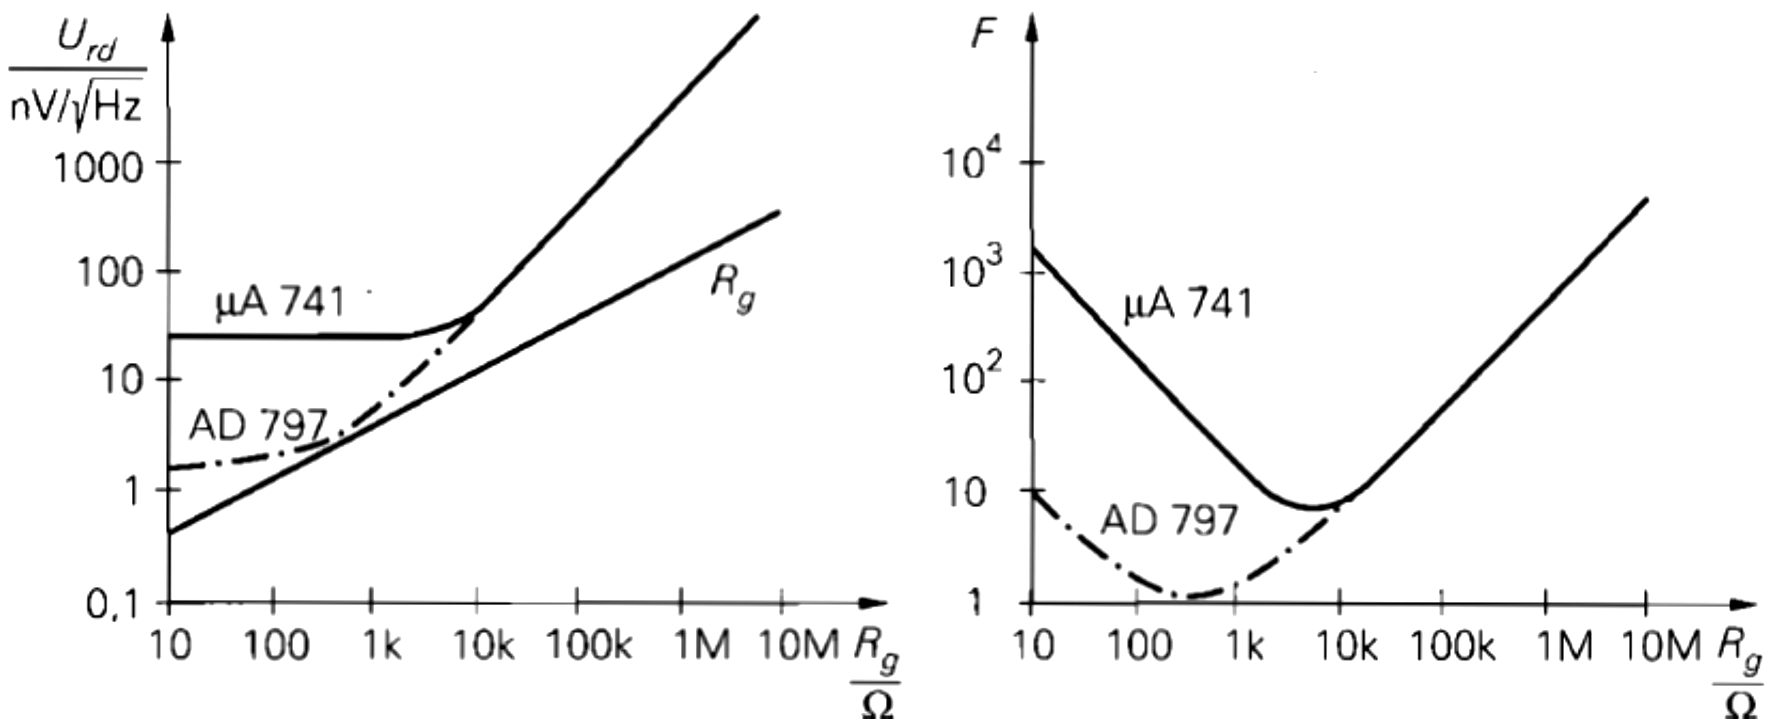
\includegraphics[width=0.75\textwidth]{images/NoiseSourceResistance.png}
				\caption{Noise as a function of source resistance}
				\label{Fig:NoiseSourceResistance}
			\end{figure}
			
		\subsubsection{Voltage and current noise performances}
			CMOS circuits tend to have less current but more voltage noise.\\
			They also tend to have higher noise corner frequencies.  
			\begin{figure}[h]
				\centering
				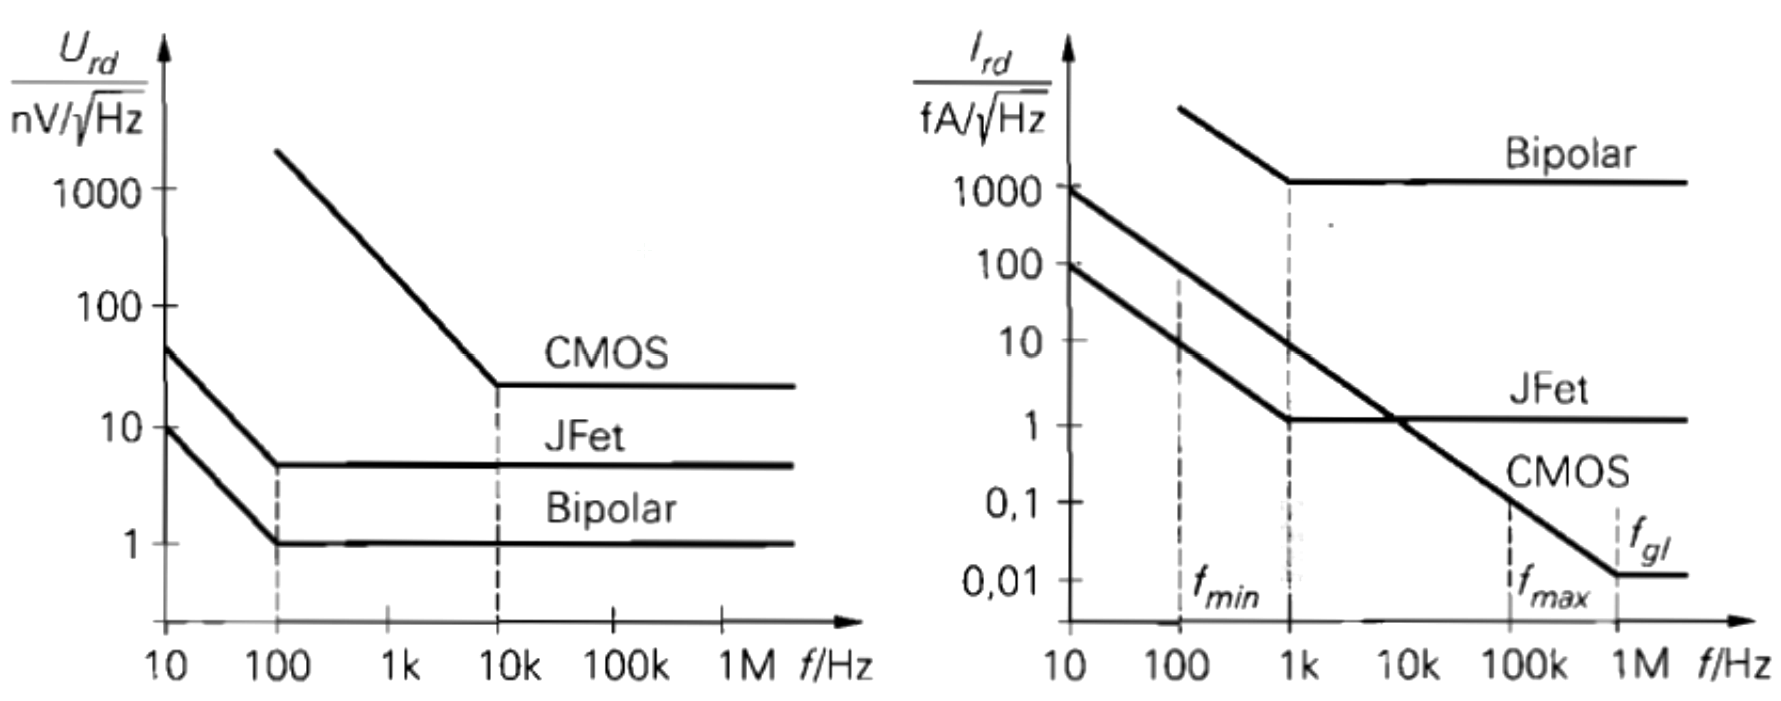
\includegraphics[width=0.75\textwidth]{images/VoltageCurrentNoise.png}
				\caption{Noise performance of voltage and current}
				\label{Fig:VoltageCurrentNoise}
			\end{figure}
			
		\subsubsection{Auto-Zero Principle}
			Measure input offset and subtract it from input in order to cancel low frequency noise density increase. 
			The measured offset is stored in a capacitor, which discharge must be much slower than the offset measurement period $T_{AZ}$ $\rightarrow$ $RC >> T_{AZ}$! 
			\begin{figure}[h]
				\centering
				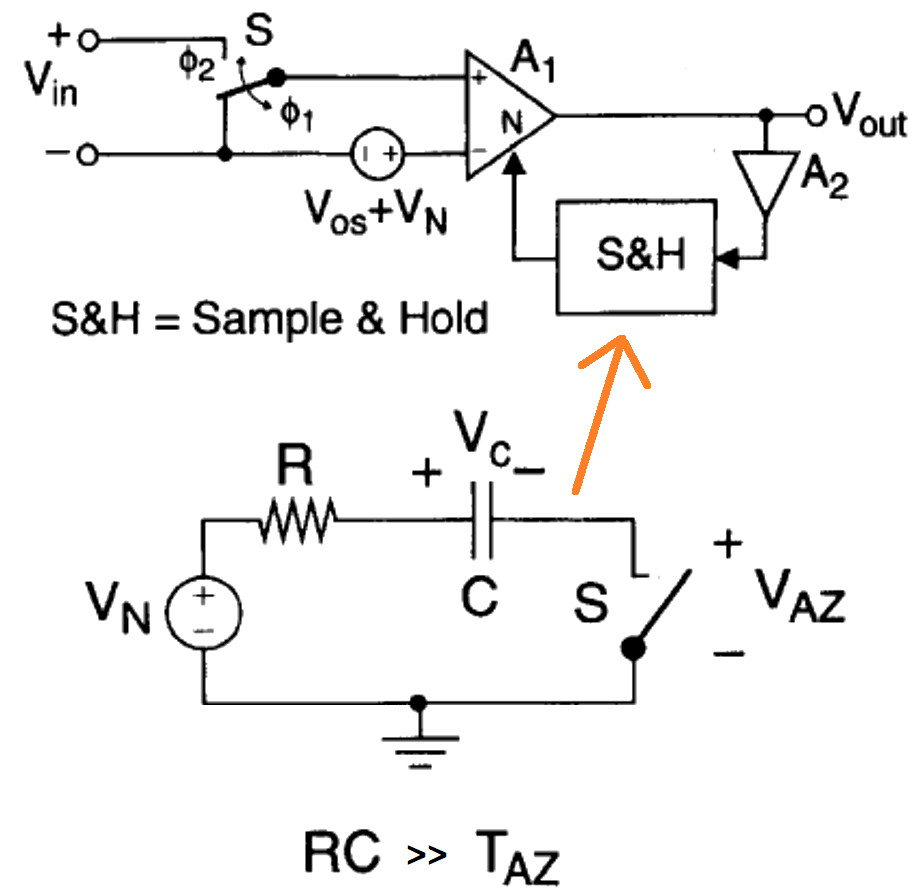
\includegraphics[width=0.35\textwidth]{images/AutoZeroPrinzip.png}
				\caption{Auto-Zero Principle}
				\label{Fig:AutoZeroPrinzip}
			\end{figure}
			\\
			There is the possibility of open-loop or closed-loop cancellation, where in the closed-loop cancellation the offset is stored on a floating capacitor which is more precise in switched capacitor circuits. For the schematic of the closed- and open-loop cancellation please refer to slide 16 in OPAMP2. \\
			\textbf{Disdvantage of auto-zeroing} is that during the measurement the principal function of the circuit is not operating. However, two parallel amp stages avoid this problem, where the null amp measures the offset of the main amp online. See slide 17 in OPAMP2 for schematic. 
			
		\subsubsection{Chopper Amp}
			The chopper amp is used for amplifying weak DC and low-frequency signals. The principle is that the given signal is chopped and modulated to a higher frequency where it is amplified and downconverted again to the lower frequency, this principle helps to avoid the disturbing 1/f noise in the low frequency area. 
			
			\begin{table}[h!]
				\centering
				\begin{tabular}{m{0.45\textwidth} m{0.35\textwidth} }
					
					\begin{center}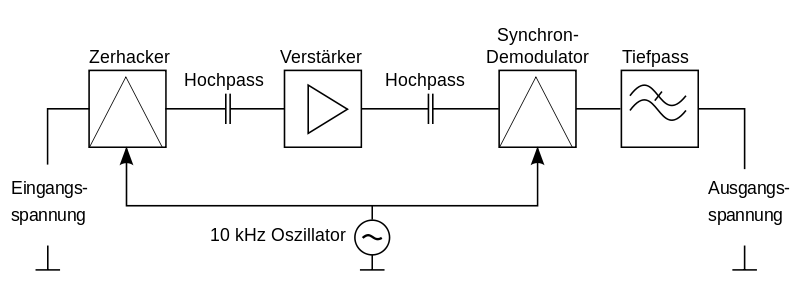
\includegraphics[width=0.35\textwidth]{images/ChopperAmp.png}\end{center} 
				&
							
					\begin{center}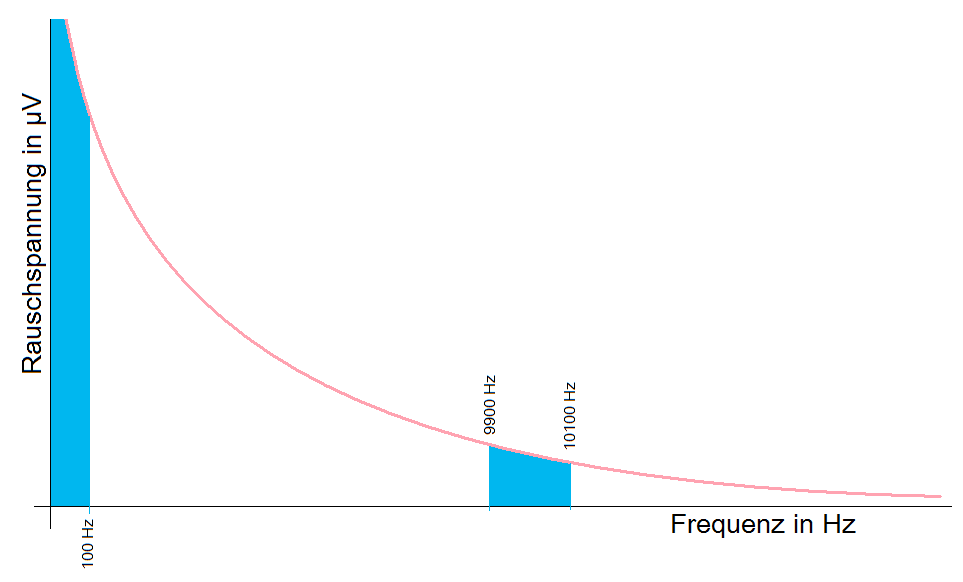
\includegraphics[width=0.35\textwidth]{images/Chopperrauschen.png}\end{center} 
				\\
			
				\end{tabular}
			\end{table}			
		
	\subsection{Amplifier Types}
		\subsubsection{Transconductance Amplifier - VC Amp}
			This voltage controlled amplifier converts a differential voltage on its input into a proportional current on the output. In contrary to normal OPAMPs the OTA (operational transconductance amp) has a high impedance output, meaning that the output voltage depends mainly on the given load. 
			The gain is given by the equation below, where $U_a$ is the output voltage, $U_D$ is the differential voltage, $R_a$ is the external load resistor and $g_m$ is the conductance of the amplifier. 
			\begin{table}[h!]
				\centering
				\begin{tabular}{m{0.45\textwidth} m{0.35\textwidth} }
					
					\begin{equation}
						G = \frac{U_a}{U_D} = R_a g_m
					\end{equation}		
				&
							
					\begin{center}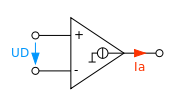
\includegraphics[width=0.25\textwidth]{images/OTA.png}\end{center} 
				\\
			
				\end{tabular}
			\end{table}
			\\
			Applications: \\
			\begin{itemize}
				\setlength{\itemsep}{-4pt}
				\item Realization of analog filters without ohmic resistance
				\item Coax line driver (the high output resistance helps to avoid reflections)
				\item Etc.
			\end{itemize}			
			
		\subsubsection{Transimpedance Amplifier - CV Amp}
			This current controlled amplifier converts an input current into an equivalent voltage on the output. The formula below gives the gain of the transimpedance amp, where $Z$ is the transimpedance and $r_s$ is the output resistance at negative input.  
			\begin{table}[h!]
				\centering
				\begin{tabular}{m{0.75\textwidth}}
					
					\begin{equation}
						G = \frac{U_a}{U_D} = \frac{Z}{r_s}
					\end{equation}	

				\\
							
					\begin{center}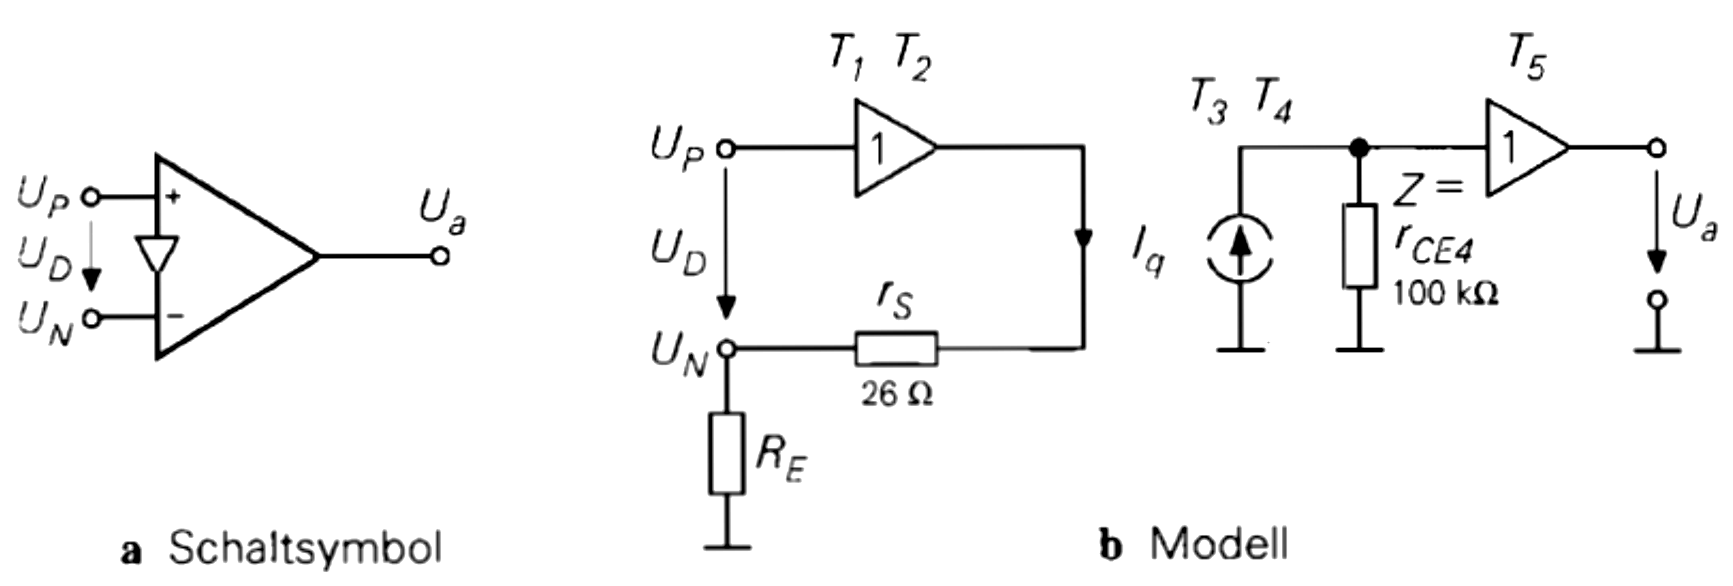
\includegraphics[width=0.55\textwidth]{images/TransimpedanceOPAMPModell.png}\end{center} 
				\\
			
				\end{tabular}
			\end{table}
			\\
			Applications: \\
			\begin{itemize}
				\setlength{\itemsep}{-4pt}
				\item Measurement of very small currents (for instance photo currents), it is possible to measure in the nano ampere range
				\item As voltage follower or as a compensation for the low pass behaviour of loop gain
			\end{itemize}
			
		\subsubsection{Current Amplifier - CC Amp}
			This amplifier - also called diamond transistor - acts like an ideal bipolar transistor, it has a low ohmic inverting current input and a high ohmic current output. The collector current is equal to the emitter current, whereas the base input resistance is high, the emitter input resistance is low and the collector output resistance is high. \\
			However there are some differences to a normal transistor, the collector current is - as mentioned before - inverted, $U_{BE} = 0$, the operating point is defined internally and the emitter and collector currents can flow in both directions.  
			\begin{table}[h!]
				\centering
				\begin{tabular}{m{0.75\textwidth}}
					
					\begin{equation}
						G = \frac{R}{r_s+R_E}
					\end{equation}	

				\\
							
					\begin{center}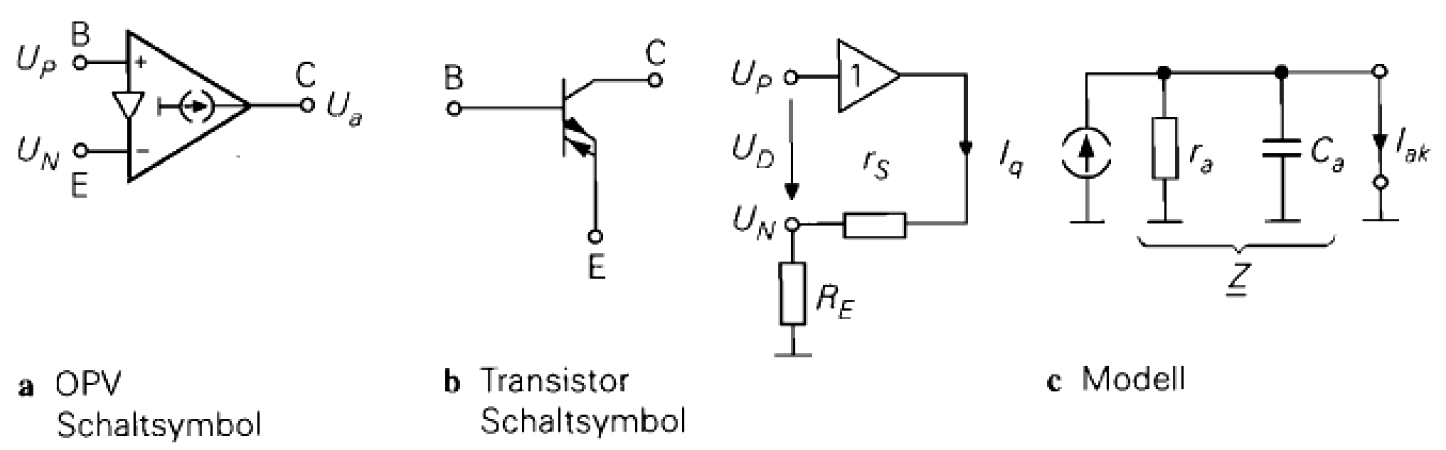
\includegraphics[width=0.55\textwidth]{images/CurrentAmp.png}\end{center} 
				\\
			
				\end{tabular}
			\end{table}
			\\
			Applications: \\
			\begin{itemize}
				\setlength{\itemsep}{-4pt}
				\item Emitter Coupling : Emitter circuit followed by collector circuit to avoid influence of load on gain (see slide 12 in OPAMP3).
				\item Collector Coupling: No idea... but if you connect the collector with the emitter you get twice the output current which is nice (but half the output resistance) (see slide 13 in OPAMP3).
				\item Base Coupling: Can be used in order to add or subtract signals (see slide 14 in OPAMP3).
				\item Difference amplifier with two current amps: Get a high bandwidth precision rectifier (slide 15).
				\item Gyrator: Dual of a transformer (slide 16).
				\item Integrator: Build a non inverting integrator with a high upper frequency limit (slide 17).
				\item Second order band-/low-pass filter (slide 18).
				\item Active Termination: The power dissipation in the feedback resistor is reduced compared with a VC amplifier (slide 18).
			\end{itemize}
	
	\subsubsection{Transistor basics}
			
		\includegraphics[
			trim=2cm 4.4cm 2cm 19cm, %l b r t
			clip=true,
			width=1.0\textwidth,
			keepaspectratio,
			angle=0,
			page=28
			]{images/Elo2_Kap1_Bipo-Transistor.pdf}
			
		\includegraphics[
			trim=2cm 20cm 2cm 4.6cm, %l b r t
			clip=true,
			width=1.0\textwidth,
			keepaspectratio,
			angle=0,
			page=30
			]{images/Elo2_Kap1_Bipo-Transistor.pdf}	
			
		\includegraphics[
			trim=2cm 18cm 2cm 3.5cm, %l b r t
			clip=true,
			width=1.0\textwidth,
			keepaspectratio,
			angle=0,
			page=29
			]{images/Elo2_Kap1_Bipo-Transistor.pdf}
	
		\includegraphics[
			trim=2cm 4.4cm 2cm 3.9cm, %l b r t
			clip=true,
			width=1.0\textwidth,
			keepaspectratio,
			angle=0,
			page=9
			]{images/Elo2_Kap2_Grundschaltungen_des_BT.pdf}
					
		\includegraphics[
			trim=1.5cm 2cm 2.8cm 3.2cm, %l b r t
			clip=true,
			width=1.0\textheight,
			keepaspectratio,
			angle=90,
			page=10
			]{images/Elo2_Kap2_Grundschaltungen_des_BT.pdf}
